\section{Natural Language Understanding}
A Natural Language Understanding (NLU) system should process human generated text (or speech) at a deep semantic level, represent the semantics
of the processed inputs, and reason over them to perform well at a given task. The effectiveness of NLU systems is often measured in terms of their
performance at the intended task. The inherent assumption\footnote{We rely on this assumption throughout this thesis. While interpreting the encoded
representations to test this assumption is also an active research topic, it is beyond the scope of this thesis.} behind taking a task-oriented approach
towards building NLU systems is that an improvement in the task performance correlates with an improvement in the quality of the semantic representation,
or in other words, the understanding capability of the computational system.

NLU is thus an umbrella term that includes several tasks, that can be defined in terms of their end goals. For example, Question Answering (QA) refers to answering questions about a span of text,
or other structured knowledge representations like knowledge bases or even images.
QA systems are required to encode the meaning of the provided inputs such that the relevant bits of information can be retrieved to answer questions.
Recognizing Textual Entailment (RTE), another NLU task, refers to the problem of identifying whether the truth value of some text provided as a hypothesis follows from that of another 
text provided as a premise, and it is usually done by extracting relevant features from the hypothesis and the premise to see if there is enough
overlap between them in the right direction. Another NLU task is Sentiment Analysis, which requires automatically categorizing the opinions expressed in the input
utterances towards specific targets. This involves extracting appropriate affective states and subjective information, such that a sentiment classifier
can be built using that information as features. To perform well at at each of these tasks, the NLU system should encode the semantics of the input to support the
kind of reasoning appropriate for the task.

In each of the examples above, it can be noticed that there are two common components: an \textbf{encoder} and a \textbf{predictor}. The encoder
extracts task-relevant features from the input, and the predictor performs the appropriate computation on top of the features given by the encoder
to produce the desired result. A generic NLU system can thus be succinctly described using the
following two equations.
\begin{align}
 \mathbf{e} &= \mathtt{encode}(\mathbf{I}) \label{eq:generic_encoding}\\
 \mathbf{o} &= \mathtt{predict}(\mathbf{e}) \label{eq:generic_prediction}
\end{align}
where $\mathbf{I}$ is the set of textual inputs to the NLU system. 
For example, $\mathbf{I}$  are single sentences in Sentiment Analysis and pairs of sentences in RTE. $\textbf{e}$ are intermediate 
encoded representations of the inputs (which may or may not be task specific), and $\mathbf{o}$ are the final task specific predictions. For example, in Sentiment Analysis or RTE, 
$\mathbf{o}$ are categorical labels indicating the sentiment or entailment respectively, and in the case of Semantic Parsing, they are structured outputs, called parses.

%TODO: Ed:"this paragraph needs a lot more detail"
In older feature-rich methods for NLU, 
Equation~\ref{eq:generic_encoding} is a mapping of the inputs to a hand designed feature space, typically containing patterns over word classes based on
part-of-speech \citep{corley2005measuring} or Wordnet synsets \citep{moldovan2001logic}; shallow linguistic features like dependencies \citep{bos2005recognising};
named entity information \cite{tatu2005semantic}; or other features depending on the task. The choice of features was left to the discretion of the ML-practitioners
designing the NLU systems. In such systems, the modeling emphasis was more on the prediction component, and the encoding component did not involve any learning. 
More recent systems \citep[among many others]{bahdanau:14,weston2014memory,hermann2015teaching,Xiong2016DynamicMN,bowman2016fast,yang:16} 
use representation learning or deep learning techniques to also learn the parameters of the
$\mathtt{encode}$ function, and typically this is done jointly with learning the parameters of the $\mathtt{predict}$ function, to ensure task-relevancy of the learned representations.

\section{Knowledge}
\label{sec:intro_external_knowledge}
A computational system that seeks to understand human utterances, cannot do so given the utterances alone. This is because, the utterances themselves
seldom contain all the information needed to comprehend them. The missing information is either part of the background knowledge about the world humans
inherently possess, or contained in the surrounding context in which the utterance is spoken or written. NLU systems thus need to access or infer this knowledge
to comprehend human languages.

In this thesis, we draw a distinction between the two kinds of knowledge described here: background and contextual. We now describe them in the context of NLU.

\subsection{Background Knowledge}
An issue with the formulation of the problem in Equation~\ref{eq:generic_encoding} is that it is missing a key input: \textbf{background knowledge}. 
Since human language is aimed at other humans who share 
the same background knowledge, a lot of information is often not explicitly stated
for the sake of brevity. The implicit knowledge required to understand language varies 
from simple commonsense in the case of basic conversations, to domain specific knowledge
about concepts in more esoteric or technical communications.

The notion of implicit knowledge can be illustrated using the following example. Consider the
events described by the following three sentences:

\begin{itemize}
 \item[] \textit{Cops shoot a man.}
 \item[] \textit{Man shoots a dog.}
 \item[] \textit{Dog shoots a man.}
\end{itemize}

Clearly, one would find the third sentence more unusual compared to the first and the second, the reason being that
a \emph{dog} performing a \emph{shooting} action does not agree with our knowledge about the general state
of affairs. While this information is not clearly written down anywhere, humans know it implicitly. An NLU
system that is designed to differentiate between these sentences should be provided with the information
that \emph{dog} in the role of the agent for \emph{shooting} is unlikely, while it can be the patient for
\emph{shooting}, and \emph{man} fits equally well as agent and patient for \emph{shooting}. The notion that
some combinations of actions and their arguments are more semantically likely than others is referred to as
Selectional Preference \citep{wilks1973preference}, and we describe that in greater detail in Chapter~\ref{chapter:nem}.

Consider another example of the need for encoding commonsense information, that of solving the 
textual entailment problem given the following premise and candidate hypothesis:
\begin{itemize}
 \item[] \textbf{Premise:} \textit{Children and parents are splashing water at the pool.}
 \item[] \textbf{Hypothesis} \textit{Families are playing outside.}
\end{itemize}
The knowledge a human uses to correctly predict that the hypothesis can be inferred from the 
premise is that \textit{children and parents} typically form \textit{families}, \textit{splashing water} 
is a kind of \textit{playing}, and a \textit{pool} is expected to be \textit{outside}. An entailment model trained on texts like the
ones shown above, with just the sentences as inputs, will not have access to the background knowledge that humans possess.
% TODO: Give a PPA example here?
Such a model will at best memorize co-occurrence patterns in the input words. Using pre-trained vectors to represent input words provides additional
knowledge to the model in the form of co-occurrence statistics obtained from large corpora. However, it is unclear whether distributional
information at the word level alone can substitute for the kind of knowledge described above.
Fortunately, background knowledge of this kind is encoded to some extent in machine readable
ontologies and knowledge bases.

In this thesis, we will show how such background knowledge can be encoded either by leveraging Selectional Preferences
or by incorporating external knowledge sources, and used in conjunction with distributional models to obtain better input representations
for NLU systems.

\subsection{Contextual Knowledge}
A second issue with the generic NLU formulation, particularly with Equation~\ref{eq:generic_prediction}, is that it does not take into account the context
in which the input utterance occurs. Typically, context includes the circumstances that form the setting for the input utterances to be fully understood,
and hence it significantly contributes to the meaning of the inputs.
%TODO: Ed: "There are several types of contexts: co-text, situational, political, environmental..."
In this thesis, we will refer to this additional information as \textbf{contextual knowledge}.
Unlike background knowledge, this is not implicit in the
text being read. However, reasoning in the presence of contextual knowledge still poses significant challenges. An automated reading comprehension system that
reasons over this additional information is expected to effectively do the following: encode the context in such a way that the bits of information relevant to the input
utterances can be aligned to the input; encode the inputs in such a way that they can be executed against the encoded context to produce the desired output. Approaches
for encoding inputs and contexts, and linking them depend on the nature of the contextual information.

%TODO: The following paragraph needs to be improved.
In the case of structured contexts, such as knowledge graphs, linking contexts
to inputs is referred to as \emph{entity linking}, and encoding inputs is a \emph{Semantic Parsing} problem, where the natural language utterances are translated into
logical forms that can be executed against the knowledge graph to produce the desired output.
% TODO: Give examples of semantic parsing papers.
When the contexts are unstructured, the problem boils down to encoding the context in a way to facilitate extracting input-specific information from it. This is usually
referred to as \emph{Information Extraction}.
Examples include \cite{hill2015goldilocks,richardson2013mctest,penas2013qa4mre,breck2001looking}.
In this thesis, we focus on both structured and unstructured contexts.

Figure~\ref{fig:wikitables_example} shows a question taken from the Wikitables dataset \citep{pasupat2015compositional}, and an associated table from a Wikipedia article,
which provides the necessary context to answer it. This an example of a QA task where the context is (semi) structured. As it can be seen from the example, answering this
question requires doing multi-step reasoning over the table.
\begin{figure}
\begin{center}
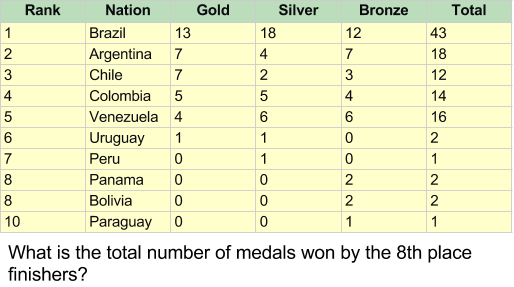
\includegraphics[width=4in]{figures/wikitables_example.png}
\caption{Example of a task requiring reasoning over semi-structured context}
\label{fig:wikitables_example}
\end{center}
\end{figure}

Figure~\ref{fig:babi_example} shows an example where the context is unstructured. This is from the bAbI dataset \citep{weston2015towards}, which is a collection of artificially generated toy tasks.
The first six sentences in the example
form the context, and the final line is a question followed by the answer and pointers to the relevant sentences in the context. A QA system is expected to learn to find the appropriate context
given the question and answer it correctly.
\begin{figure}
\begin{center}
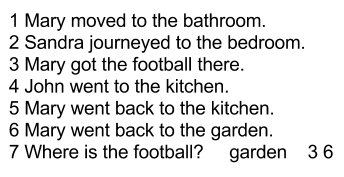
\includegraphics[width=3in]{figures/bAbI_example.png}
\caption{Example of an artificial task requiring reasoning over context, part of the bAbI dataset}
\label{fig:babi_example}
\end{center}
\end{figure}

Figure~\ref{fig:science_qa_example} shows a relatively more difficult QA example from Aristo science question answering dataset \citep{clark2015elementary}. Simple techniques such as measuring lexical overlap do not
work well for this task because all four options have significant overlap with the sentences in context. As we show in Chapter~\ref{chapter:memnet_qa}, this task requires modeling complex entailment to be able to match the information present in the context with that in the question and
option pairs.
\begin{figure}
\begin{center}
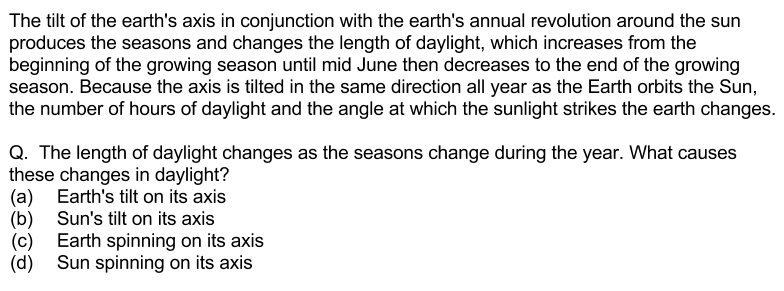
\includegraphics[width=6in]{figures/science_qa_example.png}
\caption{Snippet from a science textbook followed by a question}
\label{fig:science_qa_example}
\end{center}
\end{figure}


\section{Knowledge-Aware NLU}
Given that knowledge, both background and contextual, plays an important role in several real-world language understanding tasks, we need to reconsider
our definition of the generic NLU pipeline.
Without background knowledge, the encoding of inputs will be incomplete, and the NLU systems might not generalize beyond the specific patterns 
seen in the training data to unseen test cases. Without contextual knowledge, and an effective method to link encoded inputs to contexts, the NLU
systems will simply not have sufficient information to produce the desired results. We thus modify our NLU equations as follows.
\begin{align}
 \mathbf{e} &= \mathtt{encode\_with\_background}(\mathbf{I}, \mathbf{K}_e) \label{eq:encoding_with_knowledge}\\
 \mathbf{e}_{K_p} &= \mathtt{encode\_context}(\mathbf{K}_p) \\ \label{eq:knowledge_encoding}
 \mathbf{o} &= \mathtt{predict\_in\_context}(\mathbf{e}, \mathbf{e}_{K_p}) \label{eq:prediction_with_knowledge}
\end{align}
where $\mathbf{K}_e$ and $\mathbf{K}_p$ represent the knowledge required for encoding and prediction respectively. They
come from different sources and augment the inputs in different ways.

Obtaining relevant background or contextual
knowledge can be challenging as well, depending on the task being solved. In this thesis, we do not put a lot of emphasis on these
problems, except in Chapter~\ref{chapter:memnet_qa}, where we focus on context retrieval. In the remaining chapters, we will focus on tasks
and datasets where obtaining appropriate knowledge is easy.

\paragraph{Better encoding with background knowledge}
$\mathbf{K}_e$ is additional knowledge used to fill in the semantic gaps in the inputs, and thus obtain better
encoded representations of them. One source of such background knowledge is knowledge bases and ontologies, which encode
it explicitly. Examples include hypernym trees from WordNet for incorporating sense and generalization information about
concepts while composing sentences and subgraph features from Freebase to encode relations
between entities seen in the input text. \cite{moldovan2001logic} and \cite{krymolowski1998incorporating} are examples of a feature-rich systems that encoded input sentences in the 
context of external knowledge. Both systems used WordNet features and other related information about the semantic classes of the words in the input in NLU tasks. While \cite{krymolowski1998incorporating} 
built a system based on SNoW \citep{CCRR99} for predicting Prepositional Phrase Attachment, \cite{moldovan2001logic} built a QA system. In Chapter~\ref{chapter:ontolstm} we describe
a representation-learning application of knowledge-aware encoding where we show the advantages of incorporating WordNet information in recurrent neural networks for encoding sentences.

Such explicit sources of knowledge are often incomplete, or may not contain the kind of knowledge needed to fill the gaps to obtain representations need for the task at hand. 
An alternative source of background knowledge is a model of selectional preferences \citep{wilks1973preference}, given an appropriate structured representation of the inputs.
We exploit the idea that predicates place certain constraints on the semantic content of their arguments, and some predicate-argument structures are more common than others.
Accordingly, we model the co-occurrences within the appropriate structures to model these preferences. In Chapter~\ref{chapter:nem}, we explain this idea in greater detail
and leverage selectional preferences in SRL structures to build an NLU system that understands events in the newswire domain.

\paragraph{Reasoning with contextual knowledge}
$\textbf{K}_p$ inputs allow the prediction step to reason using additional contextual knowledge. $\textbf{K}_p$ can either be structured or unstructured. In cases where the prediction component
needs to learn to perform a sequence of operations (or a program), to arrive at the required output, the prediction becomes a Semantic Parsing problem.
The contexts are often structured in this case. There exist both traditional \citep[among others]{Zelle1996LearningTP,Zettlemoyer2005LearningTM,zettlemoyer2007online} and neural network based methods
\citep{Dong2016LanguageTL,Andreas2016LearningTC,Liang2016NeuralSM,Neelakantan2016LearningAN} for solving these problems. 
In this thesis, we build on top of this work on Semantic Parsing, and describe a type driven neural semantic 
parsing framework in Chapter~\ref{chapter:nnsp}, where we assume only weak supervision in the form of question answer pairs, and not the programs.

Machine reading comprehension typically involves encoding some context given as a paragraph and using it to
produce an answer from an encoded question. Examples of task targeted datasets built to evaluate that capability include MCTest \citep{Richardson2013MCTestAC},
CNN/Daily Mail dataset \citep{hermann2015teaching}, SQuAD \citep{Rajpurkar2016SQuAD10} and TriviQA \citep{Joshi2017TriviaQAAL}, among others.
Systems built for these tasks including attentive readers \citep{hermann2015teaching}, variants of memory networks \citep{weston2014memory,Sukhbaatar2015EndToEndMN,Xiong2016DynamicMN}
and the more recent Bidirectional Attention Flow \citep{Seo2016BidirectionalAF} can be viewed as different instantiations
of the $\mathtt{predict\_with\_context}$ function, where $\textbf{K}_p$ is some background text that needs to be understood to answer a question about it. 
In Chapter~\ref{chapter:memnet_qa}, we describe a generic formulation of the problem.

\section{Challenges}
%TODO: Challenges with using selectional preferences

Adding external knowledge inputs to NLU systems is not straightforward.  Firstly, while linking text being read to some structured background knowledge
in a KB, an automated system usually faces considerable ambiguity. For example, with lexical ontologies like WordNet, 
we get useful type hierarchies like \textit{parent is-a ancestor is-a person} and \textit{pool is-a body-of-water} 
and so on, but one has to deal with sense ambiguity: \textit{pool} can also be a game. Moreover, the fact that the two sources of semantic information are fundamentally different 
makes this challenging. While distributional approaches encode meaning in a
continuous and abstract fashion, meaning in KBs is usually symbolic and discrete. Chapter~\ref{chapter:ontolstm} is dedicated to learning 
distributions over the discrete concepts of the KB conditioned on the context, to deal with exceptions in language.

%TODO: Chalenges in Semantic Parsing

When reasoning in the presence of context, finding the 
relevant parts of the provided information given the text being processed is a challenge. 
The goal of this thesis is to find the limitations of various knowledge sources --- structured and unstructured --- and use this information 
to build hybrid NLU systems that can successfully incorporate real world knowledge in deep learning models. We now describe how this thesis is organized.

\section{Thesis Outline}
\begin{figure}
\begin{center}
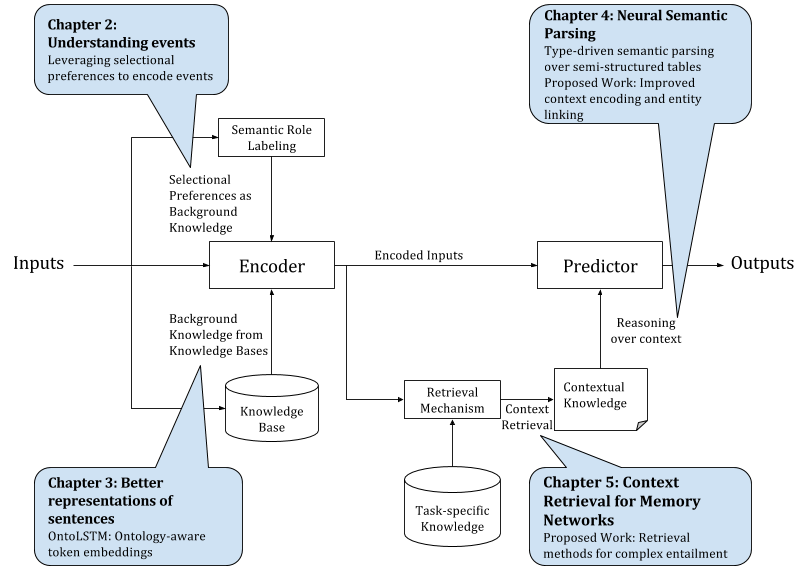
\includegraphics[width=6.5in]{figures/thesis_overview.png}
\caption{Generic NLU pipeline and thesis overview}
\label{fig:thesis_overview}
\end{center}
\end{figure}
Figure~\ref{fig:thesis_overview} shows the generic pipeline described so far, along with the breakdown of the chapters related to each component
of the pipeline.

In Chapter~\ref{chapter:nem} we encode events as predicate argument structures derived from a semantic role labeler.
In this chapter, we rely on selectional preferences between verbs and their semantic role fillers as the background
knowledge, and show how they are useful in predicting anomalous events.
Our event encoder, Neural Event Model (NEM) captures semantics deeper than the surface-level fluency. We describe an annotation effort that
resulted in newswire headlines manually labeled with the degree of surprise associated with them and show that NEM outperforms
a baseline LSTM model that encodes sentences at anomaly detection. 

In Chapter~\ref{chapter:ontolstm}, we describe a method to incorporate implicit knowledge
from WordNet towards obtaining better sentence representations. Our model looks at WordNet synsets
and at the hypernym hierarchies of the words being processed, making the 
encoder aware of their different senses and the corresponding type information.
The ontology-aware LSTM (OntoLSTM) learns to attend to the appropriate sense,
and the relevant type 
(either the most specific concept or a generalization by choosing a hypernym of
the word), conditioned on the context and the end-objective. We show that the sentence representations 
produced by OntoLSTM are better than those produced by LSTMs when used with identical prediction 
components for predicting textual entailment and preposition phrase attachment. We also visualize the attention scores assigned to the hypernyms 
of words in the input sentences and show that OntoLSTM is indeed learning useful generalizations of words
that help the learned representations perform better at the end task.

Chapter~\ref{chapter:nnsp} deals with reasoning over semi-structured contexts. We describe a type-driven
neural semantic parser aimed at answering compositional questions about Wikipedia tables. It is an encoder-decoder model that generates
well-typed logical forms that can be executed against graph representations of the tables in context. The parser also includes entity embedding
and linking modules that are trained jointly using QA supervision. This parser achieves state-of-the art result on \textsc{WikiTableQuestions} dataset.
Proposed work includes improving the entity linking module, and applying this parser to QA in other domains.

The focus of Chapter~\ref{chapter:memnet_qa} is context retrieval methods for neural network models with explicit memory components.
We start by describing a generalized deep learning architecture for reasoning over unstructured contexts. The pipeline follows the generic
specification in Section~\ref{sec:intro_external_knowledge} and has configurable components
for encoding and prediction. We identify that the memory network models in \cite{weston2014memory,Sukhbaatar2015EndToEndMN,Xiong2016DynamicMN},
the attentive reader model from \cite{hermann2015teaching}, and the Gated Attention Reader from \cite{dhingra2016gated} are specific instantiations
of our generic knowledge guided reasoning model.
Unlike prior work that evaluated these models on tasks where the contexts are limited and well-defined, we deal with tasks that require
retrieving relevant context from large corpora. Our preliminary experiments show that the choice of retrieval methods greatly affect the
final QA results. Based on this insight, we propose to build models where retrieval is tightly integrated in the QA pipeline.

% Finally, in Chapter~\ref{chapter:transfer_learning}, we propose to investigate the transferability of the representations learned for one NLU task to other tasks.
% Transfer Learning in neural networks has been well-studied in vision related tasks, and it has been established that the features learned for one task can be
% used to improve the performance of similar architectures in other tasks. Within the scope of NLU, this is a feasible investigation given that similarity
% among the neural network architectures used for various tasks. It is an important investigation because not all tasks come with lots of training data, owing to factors
% such as difficulty in getting reliable annotations and subjectivity. Moreover, with the current trend of increasing model complexity to perform better at any given task,
% it is becoming increasingly important to ensure that the models do not overfit any given dataset.